%% LyX 2.3.4.2 created this file.  For more info, see http://www.lyx.org/.
%% Do not edit unless you really know what you are doing.
\documentclass[11pt,spanish]{article}
\renewcommand{\rmdefault}{cmr}
\usepackage[T1]{fontenc}
\usepackage[utf8]{inputenc}
\usepackage{geometry}
\geometry{verbose,tmargin=2cm,bmargin=2cm,lmargin=2cm,rmargin=2cm}
\setlength{\parskip}{\bigskipamount}
\setlength{\parindent}{0pt}
\usepackage{amsmath}
\usepackage{amsthm}
\usepackage{amssymb}
\usepackage{graphicx}

\makeatletter

%%%%%%%%%%%%%%%%%%%%%%%%%%%%%% LyX specific LaTeX commands.
%% Because html converters don't know tabularnewline
\providecommand{\tabularnewline}{\\}

%%%%%%%%%%%%%%%%%%%%%%%%%%%%%% Textclass specific LaTeX commands.
\theoremstyle{definition}
\newtheorem{defn}{\protect\definitionname}[section]
\theoremstyle{definition}
\newtheorem{example}{\protect\examplename}[section]
\theoremstyle{definition}
\newtheorem{xca}{\protect\exercisename}[section]
\theoremstyle{plain}
\newtheorem{thm}{\protect\theoremname}[section]

%%%%%%%%%%%%%%%%%%%%%%%%%%%%%% User specified LaTeX commands.
\usepackage{titling}
\setlength{\droptitle}{-2cm}
\usepackage{multicol}
\usepackage{enumitem}
\usepackage{proof}
\usepackage{mathrsfs}
\usepackage{amsfonts}
\usepackage{forest}
\usepackage{ebproof}
\usepackage{amssymb}
\definecolor{Guinda}{rgb}{0.49, 0.05, 0.12}
\definecolor{Rojo}{rgb}{0.8, 0, 0}
\definecolor{Verde}{rgb}{0,0.4,0}
\definecolor{Azul}{rgb}{0,0.4,0.4}
\definecolor{Naranja}{rgb}{0.8,0.4,0}
\usepackage{tikz}
\usetikzlibrary{automata, positioning, arrows}

\makeatother

\usepackage{babel}
\addto\shorthandsspanish{\spanishdeactivate{~<>.}}

\usepackage{listings}
\lstset{mathescape=true}
\providecommand{\definitionname}{Definición}
\providecommand{\examplename}{Ejemplo}
\providecommand{\exercisename}{Ejercicio}
\providecommand{\theoremname}{Teorema}

\begin{document}
\title{Teoría de la Computación, 2021-1\\
Nota de clase 3: Autómatas Finitos}
\author{Manuel Soto Romero}
\date{\today \\ Colegio de Ciencia y Tecnología UACM}

\maketitle
\renewcommand*{\thefootnote}{\arabic{footnote}}
\setcounter{footnote}{0}
\setcounter{section}{3}
\renewcommand*\lstlistingname{C\'odigo}

\subsection{Autómatas Finitos Deterministas}

El primer tipo de máquina abstracta que estudiaremos son los Autómatas
Finitos, que permiten reconocer cadenas pertenecientes a Lenguajes
Regulares. Estos autómatas sólo pueden estar en un único estado después
de leer cualquier secuencia de entradas. Se les llama deterministas
puedes para cada entrada sólo existe uno y sólo un estado al que el
autómata puede moverse desde el estado actual.

Formalicemos esto un poco. Veamos la definición de Autómata Finito
Determinista (AFD).

\bigskip{}

\begin{defn}
\emph{(Autómata Finito Determinista) Formalmente, un Autómata Finito
Determinista (AFD) M es una quintupla $M=\left\langle Q,\Sigma,\delta,q_{0},F\right\rangle $,
donde:}
\end{defn}
\begin{itemize}
\item $Q$ \emph{es un conjunto finito de estados}
\item $\Sigma$ \emph{es el alfabeto de entrada}
\item $q_{0}$ \emph{es el estado inicial}, con $q_{0}\in Q$
\item $F$ \emph{es el conjunto de estados finales}
\item $\delta:Q\times\Sigma\rightarrow Q$ \emph{es la función de transición
entre estados, donde $\delta\left(q,a\right)=p$ se representa en
forma de diagrama o por medio de una tabla de transición.}
\end{itemize}
%
Por ejemplo, en el siguiente autómata tenemos los siguientes elementos:
\begin{itemize}
\item $\Sigma=\left\{ 0,1\right\} $
\item $Q=\left\{ q_{0},q_{1},q_{2}\right\} $
\item $q_{0}$ es el estado inicial.
\item $F=\left\{ q_{1}\right\} $
\end{itemize}
Para representar las transiciones, podemos dibujar el autómata como
un diagrama donde:
\begin{itemize}
\item Cada estado es denotado por un círculo.
\item Si un estado es inicial, tendrá una flecha que apunta hacia él sin
tener un origen.
\item Si un estado es final, se denota con un círculo doble.
\item Para pasar de un estado a otro se dibujan aristas que representan
con qué símbolo moverse.
\end{itemize}
\begin{center}
\begin{tikzpicture}[->,shorten >=1pt,auto,node distance=3cm,transform shape] 

\node[state, initial, initial text=] (S) {$q_0$}; 
\node[state, right of=S, accepting] (1) {$q_1$};
\node[state, right of=1] (2) {$q_2$};


\draw (S) edge[loop above] node{0} (S)
      (S) edge[] node{1} (1)
	  (1) edge[loop above] node{1} (1)
	  (1) edge[bend left] node{0} (2)
      (2) edge[bend left] node{0,1} (1)
;

\end{tikzpicture}
\end{center}

En este diagrama por ejemplo, supongamos que queremos leer la cadena
$011011$. Para procesarla con el autómata debemos seguir la secuencia
de estado marcada. Entonces:
\begin{enumerate}
\item Nos posicionamos en $q_{0}$, dado que nuestro primer símbolo es $0$,
no nos movemos, nos quedamos en dicho estado como indica la arista
del estado.
\item El siguiente símbolo es un $1$ que nos lleva al estado $q_{1}$.
\item El siguiente símbolo $1$ nos deja en el estado $q_{1}$.
\item El siguiente símbolo 0 nos lleva al estado $q_{2}$.
\item El siguiente símbolo 1 nos lleva al estado $q_{1}$ nuevamente.
\item El siguiente símbolo $1$ nos deja en el estado $q_{1}$.
\item Dado que acabamos de procesar todos los símbolos de la cadena y terminamos
en un estado final, podemos concluir que la cadena fue aceptada por
el autómata.
\end{enumerate}
Si no llegamos a un estado final, se dice que la cadena fue rechazada
por el autómata. Revisemos ahora, la representación de estas transiciones
como tabla:
\begin{center}
\begin{tabular}{cc|cc}
 &  & 0 & 1\tabularnewline
\hline 
$\rightarrow$ & $q_{0}$ & $q_{0}$ & $q_{1}$\tabularnewline
\textbf{F} & $q_{1}$ & $q_{2}$ & $q_{1}$\tabularnewline
 & $q_{2}$ & $q_{1}$ & $q_{1}$\tabularnewline
\end{tabular}
\par\end{center}

Con $\rightarrow$ señalamos el estado inicial y con \textbf{F }los
estados finales. 

Es importante notar que nuestra función de transición $\delta$, sólo
acepta un símbolo. Por ejemplo, para nuestro autómata anterior, tenemos:

\[
\delta\left(q_{0},1\right)=q_{1}
\]

Sin embargo, en ocasiones es útil modelar esta función de manera que
nos muestre el camino completo pasando por las transiciones, es decir,
que en lugar de recibir un símbolo, recibamos una cadena y nos muestre
dónde termina dicha cadena. Por ejemplo:

\[
\delta\left(q_{0},011011\right)=q_{1}
\]

Llamaremos a esta nueva $\delta$, la función de transición extendida
y la denotaremos por $\hat{\delta}$. Su definición es la siguiente:

\bigskip{}

\begin{defn}
\emph{(Función de Transición Extendida) La función de transición extendida,
$\hat{\delta}:Q\times\Sigma^{*}\rightarrow Q$, se define inductivamente
en términos de $\delta$ como sigue. Sea $q\in Q,a\in\Sigma$ y $x\in\Sigma^{*}$,
entonces:}
\end{defn}
\[
\begin{array}{rcl}
\hat{\delta}\left(q,\varepsilon\right) & \rightarrow & q\\
\hat{\delta}\left(q,xa\right) & \rightarrow & \delta\left(\hat{\delta}\left(q,x\right),a\right)
\end{array}
\]

Finalmente, decimos que el lenguaje de un AFD $M=\left\langle Q,\Sigma,\delta,q_{0},F\right\rangle $
denotado por $L\left(M\right)$ se define como:

\[
L\left(M\right)=\left\{ w:\hat{\delta}\left(q_{0},w\right)\in F\right\} 
\]

Es decir, son todas las cadenas que procesadas por el autómata desde
el estado inicial, terminan en un estado final.
\begin{example}
Diseñar un AFD que acepte el lenguaje

\[
L=\left\{ w:w\text{ tiene un número par de ceros y un número par de unos}\right\} 
\]

La tarea de los estados de este AFD es la de contar el número de ceros
y el número de unos contando en módulo 2. Es decir, el estado se emplea
para recordar si el número de ceros es par o impar hasta el momento
y también para recordar si el número de unos leídos hasta el momento
es par o impar. Existen por lo tanto cuatro estados que pueden interpretarse
de la siguiente forma:
\end{example}
\begin{itemize}
\item $q_{0}$: Tanto el número de ceros como el de unos leídos hasta el
momento es par.
\item $q_{1}$: El número de ceros leídos hasta el momento es par, pero
el de unos es impar.
\item $q_{2}$: El número de unos leídos hasta el momento es par, pero el
de ceros es impar.
\item $q_{3}$: Tanto el número de ceros como el de unos leídos hasta el
momento es impar.
\end{itemize}
El estado $q_{0}$ es por lo tanto el estado inicial así como el único
estado de aceptación. Es el estado inicial porque antes de leer cualquier
cosa, la cantidad de ceros y unos leídos hasta ese momento es igual
a cero y cero es par. Es el único estado de aceptación porque describe
de forma exacta la condición para que una secuencia de ceros y unos
pertenezca al lenguaje $L$.

Con esto, definimos nuestro autómata con:

\[
\left\langle \left\{ q_{0},q_{1},q_{2},q_{3}\right\} ,\left\{ 0,1\right\} ,\delta,q_{0},\left\{ q_{0}\right\} \right\rangle 
\]

Representamos la función de transición en formato de diagrama y de
tabla.

\begin{center}
\begin{tikzpicture}[->,shorten >=1pt,auto,node distance=3cm,transform shape] 

\node[state, initial, initial text=,accepting] (S) {$q_0$}; 
\node[state, right of=S] (1) {$q_1$};
\node[state, below of=S] (2) {$q_2$};
\node[state, below of=1] (3) {$q_3$};


\draw (S) edge[bend left] node{1} (1)
      (S) edge[bend left] node{0} (2)
	  (1) edge[bend left] node{0} (3)
	  (1) edge[bend left] node{1} (S)
      (2) edge[bend left] node{0} (S)
	  (2) edge[bend left] node{1} (3)
      (3) edge[bend left] node{0} (1)
	  (3) edge[bend left] node{1} (2)
;

\end{tikzpicture}
\end{center}
\begin{center}
\begin{tabular}{ccc|cc}
 &  &  & 0 & 1\tabularnewline
\hline 
\textbf{F} & $\rightarrow$ & $q_{0}$ & $q_{2}$ & $q_{1}$\tabularnewline
 &  & $q_{1}$ & $q_{3}$ & $q_{0}$\tabularnewline
 &  & $q_{2}$ & $q_{0}$ & $q_{3}$\tabularnewline
 &  & $q_{3}$ & $q_{1}$ & $q_{2}$\tabularnewline
\end{tabular}
\par\end{center}

\bigskip{}

\begin{xca}
Obtén los siguientes AFD:
\end{xca}
\begin{itemize}
\item Un AFD que dado el alfabeto $\Sigma=\left\{ 0,1\right\} $ reconozca
el lenguaje de todas las cadenas que inician en 0.
\item Un AFD que dado el alfabeto $\Sigma=\left\{ 0,1\right\} $ reconozca
el lenguaje de todas las cadenas que termian en 1.
\item Un AFD que dado el alfabeto $\Sigma=\left\{ 0,1\right\} $ reconozca
el lenguaje de todas las cadenas que contienen la subcadena 01.
\end{itemize}
%

\subsubsection{Minimización de AFD}

Al diseñar AFD, podemos tener distintas versiones que reconocen el
mismo lenguaje. Esto en un principio, no representa ningún problema,
sin embargo, podemos llegar a tener casos donde el autómata tenga
estados y/o transiciones que en realidad no son del todo esenciales.
Veamos algunos ejemplos:
\begin{itemize}
\item Analicemos por ejemplo el siguiente AFD, ¿qué lenguaje reconoce?

\begin{center}
\begin{tikzpicture}[->,shorten >=1pt,auto,node distance=2cm,transform shape] 

\node[state, initial, initial text=,below of=1] (S) {$q_0$}; 
\node[state, right of=S, above of=S,accepting] (1) {$q_1$};
\node[state, right of=S, below of=S,accepting] (2) {$q_2$};
\node[state, right of=1, below of=1] (3) {$q_3$};


\draw (S) edge[bend left] node{a} (1)
      (S) edge[bend right] node{b} (2)
	  (1) edge[bend left] node{a,b} (3)
      (2) edge[bend right] node{a,b} (3)
	  (3) edge[loop right] node{a,b} (3)
;

\end{tikzpicture}
\end{center}

Es fácil ver que el lenguaje admitido por este autómata es $\left\{ a,b\right\} $,
sin embargo, podemos notar a partir del estado $q_{0}$, que sin importar
si leemos una $a$ o una $b$, vamos a un estado final, con lo cual,
parece ser que tener dos estados no es del todo necesario. De la misma
forma, en ambos casos, una vez que llegamos a un estado de aceptación
y leer cualquier otro símbolo del alfabeto, llegamos al estado $q_{3}$
lo cual reafirma el hecho de que no es necesario tener estado diferentes.

A partir del análisis anterior, podemos modificar el autómata como
sigue:

\begin{center}
\begin{tikzpicture}[->,shorten >=1pt,auto,node distance=1cm,transform shape] 

\node[state, initial, initial text=,below of=1] (S) {$p_0$}; 
\node[state, right of=S, right of=S,accepting] (1) {$p_1$};
\node[state, right of=S, right of=1] (2) {$p_2$};


\draw (S) edge[] node{a,b} (1)
      (1) edge[] node{a,b} (2)
      (2) edge[loop above] node{a,b} (3)
;

\end{tikzpicture}
\end{center}
\item Veamos ahora el siguiente AFD, ¿qué lenguaje reconoce?

\begin{center}
\begin{tikzpicture}[->,shorten >=1pt,auto,node distance=1.5cm,transform shape] 

\node[state, initial, initial text=,below of=1] (S) {$q_0$}; 
\node[state, right of=S, above of=S,accepting] (1) {$q_1$};
\node[state, right of=S, below of=S,accepting] (2) {$q_2$};
\node[state, right of=1] (3) {$q_3$};
\node[state, right of=2] (4) {$q_4$};
\node[state, right of=3, below of=3,accepting] (5) {$q_5$};


\draw (S) edge[bend left] node{$a$} (1)
      (S) edge[bend right] node{$b$} (2)
	  (1) edge[] node{$a$} (3)
      (1) edge[] node{$b$} (4)
	  (2) edge[] node{$b$} (3)
      (2) edge[] node{$a$} (4)
      (3) edge[bend left] node{$a,b$} (5)
      (4) edge[bend right] node{$a,b$} (5)
      (5) edge[loop right] node{$a,b$} (5)
;

\end{tikzpicture}
\end{center}

Los estados $q_{1}$ y $q_{2}$ nos hacen notar que, al igual que
el autómata anterior, el lenguaje reconocido es $\left\{ a,b\right\} $,
sin embargo, al seguir analizando las transiciones, vemos que también
acepta cadenas con una longitud de al menos 3. Es decir, el lenguaje
aceptado es: 

\[
\left\{ a,b\right\} \cup\left\{ w\in\left\{ a,b\right\} ^{*}:|w|\text{ es al menos 3}\right\} 
\]

Vemos que tanto $q_{1}$ como $q_{2}$ se pueden colapsar, de la misma
forma que en el ejemplo anterior. Por otro lado, los estados $q_{3}$
y $q_{4}$ son prácticamente idénticos por lo que también podemos
colapsarlos, dejando el siguiente AFD:

\begin{center}
\begin{tikzpicture}[->,shorten >=1pt,auto,node distance=2cm,transform shape] 

\node[state, initial, initial text=,below of=1] (S) {$p_0$}; 
\node[state, right of=S, accepting] (1) {$p_1$};
\node[state, right of=1] (2) {$p_2$};
\node[state, right of=2,accepting] (3) {$p_3$};


\draw (S) edge[] node{$a,b$} (1)
      (1) edge[] node{$a,b$} (2)
      (2) edge[] node{$a,b$} (3)
      (3) edge[loop above] node{$a,b$} (3)
;

\end{tikzpicture}
\end{center}
\end{itemize}
En ambos ejemplos hemos \emph{colapsado} estados que tienen el mismo
comportamiento, es decir, son \emph{equivalentes}. Esta noción de
equivalencia y el proceso de decisión sobre si colapsar o no un par
de estados, puede realizarse algorítmicamente. Veamos la definición
de equivalencia:

\bigskip{}

\begin{defn}
\emph{(Relación de equivalencia entre estados) Dado un AFD $\left\langle Q,\Sigma,\delta,q_{0},F\right\rangle $
decimos que dos estados $p$ y $q$ están relacionados si y sólo si }

\[
\forall x\in\Sigma^{*},\widehat{\delta}\left(p,x\right)\in F\leftrightarrow\widehat{\delta}\left(q,x\right)\in F
\]

\emph{Denotamos esto como}

\[
p\approx q
\]
\end{defn}
%
Intuitivamente, esta definición nos indica tres cosas importantes:
\begin{enumerate}
\item No importa qué cadena tomemos del alfabeto, si llegamos a un estado
final partiendo de $p$ o $q$ es equivalente.
\item No necesariamente $p$ y $q$ deben ser iniciales, puede ser cualquier
estado. tampoco deben ser finales.
\item Tienen el mismo comportamiento bajo todas las cadenas posibles.
\end{enumerate}
Partiendo de esta definición, se define el \emph{algoritmo de minimización
}como sigue:
\begin{enumerate}
\item Escribir una tabla para cada uno de los pares de estados $\left\{ p,q\right\} $,
inicialmente sin marca alguna.
\item Marcar la celda correspondiente a $\left\{ p,q\right\} $ si $p\in F$
y $q\notin F$ o viceversa.
\item Repetir lo siguiente hasta que no se presenten cambios: Si existe
un par sin marca $\left\{ p,q\right\} $ tal que $\left\{ \delta\left(p,a\right),\delta\left(q,a\right)\right\} $
está marcado por alguna $a\in\Sigma$, entonces, marcamos la celda
$\left\{ p,q\right\} $.
\item Al terminar $p\approx q$ si y sólo si $\left\{ p,q\right\} $ no
tiene marca.
\end{enumerate}
Veamos cómo aplicar el algoritmo con el AFD revisado anteriormente:

\begin{center}
\begin{tikzpicture}[->,shorten >=1pt,auto,node distance=2cm,transform shape] 

\node[state, initial, initial text=,below of=1] (S) {$q_0$}; 
\node[state, right of=S, above of=S,accepting] (1) {$q_1$};
\node[state, right of=S, below of=S,accepting] (2) {$q_2$};
\node[state, right of=1, below of=1] (3) {$q_3$};


\draw (S) edge[bend left] node{a} (1)
      (S) edge[bend right] node{b} (2)
	  (1) edge[bend left] node{a,b} (3)
      (2) edge[bend right] node{a,b} (3)
	  (3) edge[loop right] node{a,b} (3)
;

\end{tikzpicture}
\end{center}

Construimos la tabla para cada par de estados en el autómata.
\begin{center}
\begin{tabular}{|c|c|c|ccc}
\multicolumn{1}{c}{$q_{0}$} & \multicolumn{1}{c}{} & \multicolumn{1}{c}{} &  &  & \tabularnewline
\cline{1-1} 
 & \multicolumn{1}{c}{$q_{1}$} & \multicolumn{1}{c}{} &  &  & \tabularnewline
\cline{1-2} \cline{2-2} 
 &  & \multicolumn{1}{c}{$q_{2}$} &  &  & \tabularnewline
\cline{1-3} \cline{2-3} \cline{3-3} 
 &  &  & $q_{3}$ &  & \tabularnewline
\cline{1-4} \cline{2-4} \cline{3-4} \cline{4-4} 
 &  &  & \multicolumn{1}{c|}{} & $q_{4}$ & \tabularnewline
\cline{1-5} \cline{2-5} \cline{3-5} \cline{4-5} \cline{5-5} 
 &  &  & \multicolumn{1}{c|}{} & \multicolumn{1}{c|}{} & $q_{5}$\tabularnewline
\cline{1-5} \cline{2-5} \cline{3-5} \cline{4-5} \cline{5-5} 
\end{tabular}
\par\end{center}

Para cada celda, marcarla si uno de los estados es final y el otro
no.
\begin{center}
\begin{tabular}{|c|c|cc}
\multicolumn{1}{c}{$q_{0}$} & \multicolumn{1}{c}{} &  & \tabularnewline
\cline{1-1} 
$\checkmark$ & \multicolumn{1}{c}{$q_{1}$} &  & \tabularnewline
\cline{1-2} \cline{2-2} 
$\checkmark$ &  & $q_{2}$ & \tabularnewline
\cline{1-3} \cline{2-3} \cline{3-3} 
 & $\checkmark$ & \multicolumn{1}{c|}{$\checkmark$} & $q_{3}$\tabularnewline
\cline{1-3} \cline{2-3} \cline{3-3} 
\end{tabular}
\par\end{center}

Ahora revisamos las celdas vacías y analizamos las transiciones con
cada uno. Por ejemplo, analicemos $\left\{ q_{0},q_{3}\right\} $.
Tenemos como alfabeto $\left\{ a,b\right\} $, de forma tal que $\delta\left(q_{0},a\right)=q_{1}$,
$\delta\left(q_{3},a\right)=q_{3}$, $\delta\left(q_{0},b\right)=q_{2},\delta\left(q_{3},b\right)=q_{3}$,
con lo cual debemos verificar si $\left\{ q_{1},q_{3}\right\} $ o
$\left\{ q_{2},q_{3}\right\} $ están marcados. Si están marcados,
marcamos la celda $\left\{ q_{0},q_{3}\right\} $. En este caso vemos
que $\left\{ q_{1},q_{3}\right\} $ sí está marcada, por lo tanto
marcamos la celda original.
\begin{center}
\begin{tabular}{|c|c|cc}
\multicolumn{1}{c}{$q_{0}$} & \multicolumn{1}{c}{} &  & \tabularnewline
\cline{1-1} 
$\checkmark$ & \multicolumn{1}{c}{$q_{1}$} &  & \tabularnewline
\cline{1-2} \cline{2-2} 
$\checkmark$ &  & $q_{2}$ & \tabularnewline
\cline{1-3} \cline{2-3} \cline{3-3} 
$\checkmark$ & $\checkmark$ & \multicolumn{1}{c|}{$\checkmark$} & $q_{3}$\tabularnewline
\cline{1-3} \cline{2-3} \cline{3-3} 
\end{tabular}
\par\end{center}

Realizando el mismo análisis vemos que no existe una celda marcada,
por lo tanto dejamos dicha celda vacía y dado que el proceso se repite
hasta que no haya cambios. Nuestra tabla final queda como 
\begin{center}
\begin{tabular}{|c|c|cc}
\multicolumn{1}{c}{$q_{0}$} & \multicolumn{1}{c}{} &  & \tabularnewline
\cline{1-1} 
$\checkmark$ & \multicolumn{1}{c}{$q_{1}$} &  & \tabularnewline
\cline{1-2} \cline{2-2} 
$\checkmark$ &  & $q_{2}$ & \tabularnewline
\cline{1-3} \cline{2-3} \cline{3-3} 
$\checkmark$ & $\checkmark$ & \multicolumn{1}{c|}{$\checkmark$} & $q_{3}$\tabularnewline
\cline{1-3} \cline{2-3} \cline{3-3} 
\end{tabular}
\par\end{center}

En este caso, nuestra única celda vacía fue $\left\{ q_{1},q_{2}\right\} $
con lo cual concluimos que

\[
q_{1}\approx q_{2}
\]

y podemos colapsar entonces dichos estados, por ejemplo, cambiando
todos las transiciones que llegaban y salían de $q_{2}$ a $q_{1}$:

\begin{center}
\begin{tikzpicture}[->,shorten >=1pt,auto,node distance=1cm,transform shape] 

\node[state, initial, initial text=,below of=1] (S) {$q_0$}; 
\node[state, right of=S, right of=S,accepting] (1) {$q_1$};
\node[state, right of=S, right of=1] (2) {$q_3$};


\draw (S) edge[] node{a,b} (1)
      (1) edge[] node{a,b} (2)
      (2) edge[loop above] node{a,b} (3)
;

\end{tikzpicture}
\end{center}

\bigskip{}

\begin{xca}
Minimiza el AFD revisado anteriormente, por medio del algoritmo descrito:\begin{center}
\begin{tikzpicture}[->,shorten >=1pt,auto,node distance=1.5cm,transform shape] 

\node[state, initial, initial text=,below of=1] (S) {$q_0$}; 
\node[state, right of=S, above of=S,accepting] (1) {$q_1$};
\node[state, right of=S, below of=S,accepting] (2) {$q_2$};
\node[state, right of=1] (3) {$q_3$};
\node[state, right of=2] (4) {$q_4$};
\node[state, right of=3, below of=3,accepting] (5) {$q_5$};


\draw (S) edge[bend left] node{$a$} (1)
      (S) edge[bend right] node{$b$} (2)
	  (1) edge[] node{$a$} (3)
      (1) edge[] node{$b$} (4)
	  (2) edge[] node{$b$} (3)
      (2) edge[] node{$a$} (4)
      (3) edge[bend left] node{$a,b$} (5)
      (4) edge[bend right] node{$a,b$} (5)
      (5) edge[loop right] node{$a,b$} (5)
;

\end{tikzpicture}
\end{center}
\end{xca}
%

\subsection{Autómatas Finitos No Deterministas}

Estos autómatas pueden estar en varios estados a la vez después de
leer cualquier secuencia de entradas. Se les llama no deterministas
pues para cada entrada sólo existe más de un estado al que el autómata
puede moverse desde el estado actual.

Formalicemos esto un poco. Veamos la definición de Autómata Finito
No Determinista (AFN).

\bigskip{}

\begin{defn}
\emph{(Autómata Finito No Determinista) Formalmente, un Autómata Finito
No Determinista (AFN) M es una quintupla $M=\left\langle Q,\Sigma,\delta,q_{0},F\right\rangle $,
donde:}
\end{defn}
\begin{itemize}
\item $Q$ \emph{es un conjunto finito de estados}
\item $\Sigma$ \emph{es el alfabeto de entrada}
\item $q_{0}$ \emph{es el estado inicial}, con $q_{0}\in Q$
\item $F$ \emph{es el conjunto de estados finales}
\item $\delta:Q\times\Sigma\rightarrow\mathcal{P}\left(Q\right)$ \emph{es
la función de transición entre estados, es decir, la salida de nuestra
función de transición es un subconjunto de $Q$. }
\end{itemize}
%
Por ejemplo, en el siguiente autómata tenemos los siguientes elementos:
\begin{itemize}
\item $\Sigma=\left\{ 0,1\right\} $
\item $Q=\left\{ q_{0},q_{1},q_{2}\right\} $
\item $q_{0}$ es el estado inicial.
\item $F=\left\{ q_{2}\right\} $
\end{itemize}
\begin{center}
\begin{tikzpicture}[->,shorten >=1pt,auto,node distance=2cm,transform shape] 

\node[state, initial, initial text=] (S) {$q_0$}; 
\node[state, right of=S] (1) {$q_1$};
\node[state, right of=1, accepting] (2) {$q_2$};


\draw (S) edge[loop above] node{0,1} (S)
      (S) edge[] node{0} (1)
	  (1) edge[] node{1} (2)
;

\end{tikzpicture}
\end{center}
\begin{center}
\begin{tabular}{cc|cc}
 &  & 0 & 1\tabularnewline
\hline 
$\rightarrow$ & $q_{0}$ & $\left\{ q_{0},q_{1}\right\} $ & $\left\{ q_{0}\right\} $\tabularnewline
 & $q_{1}$ & $\varnothing$ & $\left\{ q_{2}\right\} $\tabularnewline
\textbf{F} & $q_{2}$ & $\varnothing$ & $\varnothing$\tabularnewline
\end{tabular}
\par\end{center}

Este autómata reconoce cadenas formadas por ceros y unos que terminan
en 01. Notemos que el estado inicial $q_{0}$ puede llegar a diferentes
estados con el śimbolo cero y que además hay algunos estados que no
tienen transiciones definidas, por ejemplo $q_{1}$ con cero no tiene
transición y $q_{2}$ no tiene ninguna transición. Lo cuál es válido
pues $\varnothing$ es subconjunto de cualquier conjunto.

Por ejemplo, el siguiente diagrama muestra cómo el AFN procesa la
entrada 00101: Parte siempre de su estado inicial $q_{0}$. Cuando
lee el primero 0, el AFN puede psar al estado $q_{0}$ o $q_{1}$,
por lo que hace ambos. Estos dos hilosse indican en la segunda columna
del diagrama. 

A continuación, lee el segundo 0. El estado $q_{0}$ puede pasar de
nuevo $q_{0}$ o a $q_{1}$. Sin embargo, el estado $q_{1}$ no tiene
transición para la entrada 0, por lo que el autómata se detiene. Cuando
se produce la tercera entrada, un 1, hay que considerar las transiciones
tanto de $q_{0}$ como de $q_{1}$. Comprobamos que $q_{0}$ sólo
pasa a $q_{0}$ cuando la entrada es 1, mientras que el estado $q_{1}$
pasa sólo al estado $q_{2}$. Por tanto después de leer la secuencia,
el AFN se encuentra en los estados $q_{0}$ y $q_{2}$. Dado que $q_{2}$
es un estado final, el AFN acepta la secuencia 001.

Sin embargo, la entrada no ha terminado. La cuarta entrada, un 0,
hace el hilo de $q_{2}$ muera, mientras que $q_{0}$ va tanto a $q_{0}$
como a $q_{1}$. La última entrada, un 1, hace que $q_{0}$ permanezca
en este mismo estado y $q_{1}$ pasa al estado $q_{2}$. Como de nuevo
estamos en un estado de aceptación, la secuencia 00101 es aceptada.
\begin{center}
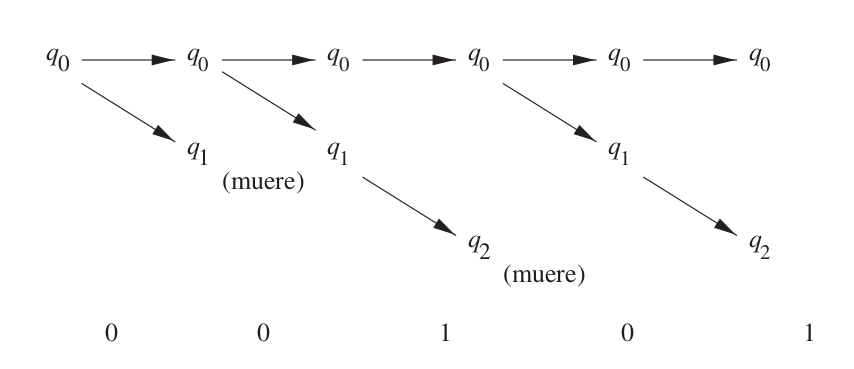
\includegraphics[scale=0.5]{imagenes/imagen1}
\par\end{center}

De manera general, diremos que una cadena es \emph{aceptada} por un
AFN si existe al menos una trayectoria de ejecución que termina en
un estado final y diremos que es \emph{rechazada} cuando todas las
posibles trayectorias de ejecución se estancan (mueren) o terminan
en un estado que no es final. Finalmente, mostramos la función de
transición extendida $\hat{\delta}$ como sigue:

\bigskip{}

\begin{defn}
\emph{(Función de Transición Extendida) La función de transición extendida,
$\hat{\delta}:Q\times\Sigma^{*}\rightarrow\mathcal{P}(Q)$, se define
inductivamente en términos de $\delta$ como sigue. Sea $q\in Q,a\in\Sigma$
y $x\in\Sigma^{*}$, entonces:}
\end{defn}
\[
\begin{array}{rcl}
\hat{\delta}\left(q,\varepsilon\right) & \rightarrow & \left\{ q\right\} \\
\hat{\delta}\left(q,xa\right) & \rightarrow & \underset{p_{i}\in\hat{\delta}(q,x)}{\text{\ensuremath{\bigcup}}}\delta\left(p_{i},a\right)
\end{array}
\]

Por ejemplo, podemos usar $\hat{\delta}$ para describir el procesamiento
de la entrada 00101 por el AFN de nuestro ejemplo anterior. 
\begin{enumerate}
\item $\hat{\delta}\left(q_{0},\varepsilon\right)=\left\{ q_{0}\right\} $
\item $\hat{\delta}\left(q_{0},0\right)=\delta\left(q_{0},0\right)=\left\{ q_{0},q_{1}\right\} $
\item $\hat{\delta}\left(q_{0},00\right)=\delta\left(q_{0},0\right)\cup\delta\left(q_{1},0\right)=\left\{ q_{0},q_{1}\right\} \cup\varnothing=\left\{ q_{0},q_{1}\right\} $
\item $\hat{\hat{\delta}\left(q_{0},001\right)=\delta\left(q_{0},1\right)\cup\delta\left(q_{1},1\right)=\left\{ q_{0}\right\} \cup\left\{ q_{2}\right\} =\left\{ q_{0},q_{2}\right\} }$
\item $\hat{\delta}\left(q_{0},0010\right)=\delta\left(q_{0},0\right)\cup\delta\left(q_{2},0\right)=\left\{ q_{0},q_{1}\right\} \cup\varnothing=\left\{ q_{0},q_{1}\right\} $
\item $\hat{\delta}\left(q_{0},00101\right)=\delta\left(q_{0},1\right)\cup\delta\left(q_{1},1\right)=\left\{ q_{0}\right\} \cup\left\{ q_{2}\right\} =\left\{ q_{0},q_{2}\right\} $
\end{enumerate}
Finalmente, decimos que el lenguaje de un AFN $N=\left\langle Q,\Sigma,\delta,q_{0},F\right\rangle $
denotado por $L\left(N\right)$ se define como:

\[
L\left(N\right)=\left\{ w\in\Sigma^{*}:\hat{\delta}\left(q_{0},w\right)\cap F\neq\varnothing\right\} 
\]

Es decir, son todas las cadenas que procesadas por el autómata desde
el estado inicial, llegan por alguna trayectoria a algún estado final. 

\bigskip{}

\begin{xca}
Obtén los siguientes AFN:
\begin{itemize}
\item Un AFN que dado el alfabeto $\Sigma=\left\{ 0,1\right\} $ reconozca
el lenguaje de todas las cadenas que inician en 0.
\item Un AFN que dado el alfabeto $\Sigma=\left\{ 0,1\right\} $ reconozca
el lenguaje de todas las cadenas que terminan en 1.
\item Un AFN que dado el alfabeto $\Sigma=\left\{ 0,1\right\} $ reconozca
el lenguaje de todas las cadenas que contienen la subcadena 01.
\end{itemize}
\end{xca}
%

\subsection{Equivalencia entre AFDs y AFNs}

El poder de un autómata se mide en términos de la habilidad para aceptar
lenguajes. Observemos que un AFD es un caso especial de un AFN, de
modo que todo lo que un AFD puede hacer, un AFN también lo puede hacer,
de hecho para cada AFN existe un AFD que acepta el mismo lenguaje.
Además, como seguramente te habrás dado cuenta, es más sencillo construir,
especificar y comprender un AFN debido a que son más concisos. En
general, los AFNs pueden ser usados para capturar patrones en procesadores
de texto, pero optamos por los AFD cuando deseamos encontrar dichos
patrones.

\bigskip{}

\begin{thm}
Para cada AFN N, existe un AFD M con $L\left(N\right)=L\left(M\right)$.
\end{thm}
%
La demostración de este teorema queda fuera de los alcances de este
curso, por lo que en su lugar, presentaremos el proceso para transformar
un AFN en un AFD por medio de la llamada \emph{construcción por subconjuntos}:
\begin{enumerate}
\item Construir una tabla de transiciones a partir del conjunto potencia,
que muestre los estados a donde se puede llegar con cada estado de
dichos conjuntos. Al conjunto que tenga como único elemento al estado
inicial, lo marcamos como final y a todos los conjunto que contengan
al estado final original, los marcamos también como finales.
\item Eliminar estados que no sean alcanzables.
\item Renombrar los estados.
\end{enumerate}
Recordemos que el conjunto potencia se define como el conjunto formado
por todos los subconjuntos de un conjunto dado. Por ejemplo, dado
el conjunto $A=\left\{ 1,2,3\right\} $, entonces 

\[
\mathcal{P}\left(A\right)=\left\{ \varnothing,\left\{ 1\right\} ,\left\{ 2\right\} ,\left\{ 3\right\} ,\left\{ 1,2\right\} ,\left\{ 1,3\right\} ,\left\{ 2,3\right\} ,\left\{ 1,2,3\right\} \right\} 
\]

Veamos entonces cómo aplicar este algoritmo con el autómata revisado
anteriormente:

\begin{center}
\begin{tikzpicture}[->,shorten >=1pt,auto,node distance=2cm,transform shape] 

\node[state, initial, initial text=] (S) {$q_0$}; 
\node[state, right of=S] (1) {$q_1$};
\node[state, right of=1, accepting] (2) {$q_2$};


\draw (S) edge[loop above] node{0,1} (S)
      (S) edge[] node{0} (1)
	  (1) edge[] node{1} (2)
;

\end{tikzpicture}
\end{center}
\begin{enumerate}
\item Construimos la tabla de transiciones a partir del conjunto potencia
\begin{itemize}
\item Inicialización:
\begin{center}
\begin{tabular}{cc|cc}
 &  & 0 & 1\tabularnewline
\hline 
 & $\varnothing$ &  & \tabularnewline
$\rightarrow$ & $\left\{ q_{0}\right\} $ &  & \tabularnewline
 & $\left\{ q_{1}\right\} $ &  & \tabularnewline
\textbf{F} & $\left\{ q_{2}\right\} $ &  & \tabularnewline
 & $\left\{ q_{0},q_{1}\right\} $ &  & \tabularnewline
\textbf{F} & $\left\{ q_{0},q_{2}\right\} $ &  & \tabularnewline
\textbf{F} & $\left\{ q_{1},q_{2}\right\} $ &  & \tabularnewline
\textbf{F} & $\left\{ q_{0},q_{1},q_{2}\right\} $ &  & \tabularnewline
\end{tabular}
\par\end{center}
\item Llenamos la tabla con los resultados de transitar desde cada uno de
los estados.
\begin{center}
\begin{tabular}{cc|cc}
 &  & 0 & 1\tabularnewline
\hline 
 & $\varnothing$ & $\varnothing$ & $\varnothing$\tabularnewline
$\rightarrow$ & $\left\{ q_{0}\right\} $ & $\left\{ q_{0},q_{1}\right\} $ & $\left\{ q_{0}\right\} $\tabularnewline
 & $\left\{ q_{1}\right\} $ & $\varnothing$ & $\left\{ q_{2}\right\} $\tabularnewline
\textbf{F} & $\left\{ q_{2}\right\} $ & $\varnothing$ & $\varnothing$\tabularnewline
 & $\left\{ q_{0},q_{1}\right\} $ & $\left\{ q_{0},q_{1}\right\} $ & $\left\{ q_{0},q_{2}\right\} $\tabularnewline
\textbf{F} & $\left\{ q_{0},q_{2}\right\} $ & $\left\{ q_{0},q_{1}\right\} $ & $\left\{ q_{0}\right\} $\tabularnewline
\textbf{F} & $\left\{ q_{1},q_{2}\right\} $ & $\varnothing$ & $\left\{ q_{2}\right\} $\tabularnewline
\textbf{F} & $\left\{ q_{0},q_{1},q_{2}\right\} $ & $\left\{ q_{0},q_{1}\right\} $ & $\left\{ q_{0},q_{2}\right\} $\tabularnewline
\end{tabular}
\par\end{center}
\item Construimos el autómata resultante

\begin{center}
\begin{tikzpicture}[->,shorten >=1pt,auto,node distance=2.3cm,transform shape] 

\node[state, initial, initial text=] (S) {$\{q_0\}$}; 
\node[state, right of=S,above of=S] (1) {$\{q_0,q_1\}$};
\node[state, right of=1,below of=1,accepting] (2) {$\{q_0,q_1,q_2\}$};
\node[state, below of=1,left of=2,accepting] (3) {$\{q_0,q_2\}$};

\node[state, right of=2] (4) {$\varnothing$};
\node[state, right of=4,above of=4] (5) {$\{q_1\}$};
\node[state, right of=5,below of=5,accepting] (6) {$\{q_2\}$};
\node[state, below of=4,left of=6,accepting] (7) {$\{q_1,q_2\}$};

\draw (S) edge[loop above] node{1} (S)
      (S) edge[] node{0} (1)
	  (1) edge[loop above] node{0} (1)
	  (1) edge[bend left] node{1} (3)
      (2) edge[] node{0} (1)
      (2) edge[] node{1} (3)
      (3) edge[bend left] node{0} (1)
      (3) edge[] node{1} (S)

      (4) edge[loop above] node{0,1} (4)
      (5) edge[] node{0} (4)
      (5) edge[] node{1} (6)
      (6) edge[] node{0,1} (4)
      (7) edge[] node{0} (4)
      (7) edge[] node{1} (6)
;

\end{tikzpicture}
\end{center}
\item Notamos que nuestro autómata se encuentra \emph{disconexo}, esto ocurre
debido a que tenemos estados inalcanzables. Partiendo desde el estado
inicial detectamos estos estados. Claramente el subautómata de la
derecha es inalcanzable, por lo tanto lo eliminamos.

\begin{center}
\begin{tikzpicture}[->,shorten >=1pt,auto,node distance=2.3cm,transform shape] 

\node[state, initial, initial text=] (S) {$\{q_0\}$}; 
\node[state, right of=S,above of=S] (1) {$\{q_0,q_1\}$};
\node[state, right of=1,below of=1,accepting] (2) {$\{q_0,q_1,q_2\}$};
\node[state, below of=1,left of=2,accepting] (3) {$\{q_0,q_2\}$};

\draw (S) edge[loop above] node{1} (S)
      (S) edge[] node{0} (1)
	  (1) edge[loop above] node{0} (1)
	  (1) edge[bend left] node{1} (3)
      (2) edge[] node{0} (1)
      (2) edge[] node{1} (3)
      (3) edge[bend left] node{0} (1)
      (3) edge[] node{1} (S)
;

\end{tikzpicture}
\end{center}

De la misma forma, el estado $\left\{ q_{0},q_{1},q_{2}\right\} $
es inalcanzable pues no hay ningún estado que llegue a él. Lo eliminamos
también.

\begin{center}
\begin{tikzpicture}[->,shorten >=1pt,auto,node distance=2.3cm,transform shape] 

\node[state, initial, initial text=] (S) {$\{q_0\}$}; 
\node[state, right of=S,above of=S] (1) {$\{q_0,q_1\}$};
\node[state, below of=1,left of=2,accepting] (3) {$\{q_0,q_2\}$};

\draw (S) edge[loop above] node{1} (S)
      (S) edge[] node{0} (1)
	  (1) edge[loop above] node{0} (1)
	  (1) edge[bend left] node{1} (3)
      (3) edge[bend left] node{0} (1)
      (3) edge[] node{1} (S)
;

\end{tikzpicture}
\end{center}
\item Finalmente, renombramos los estados.

\begin{center}
\begin{tikzpicture}[->,shorten >=1pt,auto,node distance=2.3cm,transform shape] 

\node[state, initial, initial text=] (S) {$q_0$}; 
\node[state, right of=S,above of=S] (1) {$q_1$};
\node[state, below of=1,left of=2,accepting] (3) {$q_2$};

\draw (S) edge[loop above] node{1} (S)
      (S) edge[] node{0} (1)
	  (1) edge[loop above] node{0} (1)
	  (1) edge[bend left] node{1} (3)
      (3) edge[bend left] node{0} (1)
      (3) edge[] node{1} (S)
;

\end{tikzpicture}
\end{center}
\end{itemize}
\end{enumerate}
Notamos que el autómata resultante es un AFD y que además reconoce
el mismo lenguaje: cadenas que terminen con 01.

\bigskip{}

\begin{xca}
Mediante construcción por subconjuntos, transforma el siguiente AFN
a AFD. ¿Qué lenguaje reconoce?
\end{xca}
\begin{center}
\begin{tikzpicture}[->,shorten >=1pt,auto,node distance=2cm,transform shape] 

\node[state, initial, initial text=] (S) {$q_0$}; 
\node[state, right of=S,accepting] (1) {$q_1$};
\node[state, right of=1] (2) {$q_2$};
\node[state, right of=2, accepting] (3) {$q_3$};


\draw (S) edge[loop above] node{$a$} (S)
      (S) edge[] node{$a,b$} (1)
	  (1) edge[loop above] node{$b$} (1)
      (1) edge[] node{$a$} (2)
      (2) edge[loop above] node{$a,b$} (2)
      (2) edge[] node{$b$} (3)
;

\end{tikzpicture}
\end{center}

\subsection{Equivalencia entre Autómatas Finitos y Gramáticas Regulares}

Al igual que entre los AFDs y AFNs existe una equivalencia, también
existe una equivalencia entre las gramáticas. El procedimiento de
transformación es bastante simple:
\begin{itemize}
\item Se deben asociar a los símbolos terminales de la gramática (las variables)
los estados de un autómata. Así, para cada regla $A\rightarrow bC$
en la gramática tenemos una transición $\delta\left(A,b\right)=C$.
Observemos que las variables se comportan como estados.
\item Para las reglas de constantes como $A\rightarrow b$ se generan transiciones
$\delta\left(A,b\right)=Z$ donde $Z$ es un nuevo estado para el
que no hay un símbolo terminal asociado; $Z$ es un estado final del
autómata.
\end{itemize}
Por ejemplo, supongamos la siguiente gramática:

\[
\begin{array}{rcl}
S & \rightarrow & aA\\
S & \rightarrow & bA\\
A & \rightarrow & aB\\
A & \rightarrow & bB\\
A & \rightarrow & a\\
B & \rightarrow & aA\\
B & \rightarrow & bA
\end{array}
\]

Tenemos las siguientes transiciones:

\[
\begin{array}{rcl}
\delta\left(S,a\right) & = & A\\
\delta\left(S,b\right) & = & A\\
\delta\left(A,a\right) & = & B\\
\delta\left(A,b\right) & = & B\\
\delta\left(A,a\right) & = & Z\\
\delta\left(B,a\right) & = & A\\
\delta\left(B,b\right) & = & A
\end{array}
\]

Quedando el siguiente diagrama:

\begin{center}
\begin{tikzpicture}[->,shorten >=1pt,auto,node distance=2cm,transform shape] 

\node[state, initial, initial text=] (S) {$S$}; 
\node[state, right of=S] (1) {$A$};
\node[state, right of=1] (2) {$B$};
\node[state, below of=1, accepting] (3) {$Z$};


\draw (S) edge[] node{$a,b$} (1)
      (1) edge[bend left] node{$a,b$} (2)
	  (1) edge[] node{$a$} (3)
      (2) edge[bend left] node{$a,b$} (1)
;

\end{tikzpicture}
\end{center}

El proceso inverso es similar. Basta con revisar las transiciones
de manera que si tenemos una transición $\delta\left(q_{0},a\right)=q_{1}$,
entonces tenemos una regla de producción $Q_{0}\rightarrow aQ_{1}$
y además si tenemos una transición $\delta\left(q_{1},a\right)=q_{2}$
con $q_{2}\in F$, entonces tenemos una regla $Q_{1}\rightarrow a$.
Por ejemplo, la gramática por el siguiente autómata:

\begin{center}
\begin{tikzpicture}[->,shorten >=1pt,auto,node distance=2cm,transform shape] 

\node[state, initial, initial text=, accepting] (0) {$q_0$}; 
\node[state, right of=0, accepting] (1) {$q_1$};
\node[state, right of=1, accepting] (2) {$q_2$};
\node[state, right of=2] (3) {$q_3$};


\draw (0) edge[bend left] node{$a$} (1)
      (0) edge[loop above] node{$b$} (0)
	  (1) edge[] node{$a$} (2)
      (1) edge[bend left] node{$b$} (0)
      (2) edge[] node{$a$} (3)
      (2) edge[bend left=50] node{$b$} (0)
      (3) edge[loop above] node{$a,b$} (3)
;

\end{tikzpicture}
\end{center}

tenemos las siguientes reglas, obtenidas a partir de las transiciones:

\[
\begin{array}{rclcrcl}
\delta\left(q_{0},a\right) & = & q_{1} &  & Q_{0} & \rightarrow & aQ_{1}\\
\delta\left(q_{0},b\right) & = & q_{0} &  & Q_{0} & \rightarrow & bQ_{0}\\
\delta\left(q_{0},a\right) & = & q_{1} &  & Q_{0} & \rightarrow & a\\
\delta\left(q_{0},b\right) & = & q_{0} &  & Q_{0} & \rightarrow & b\\
\delta\left(q_{1},a\right) & = & q_{2} &  & Q_{1} & \rightarrow & aQ_{2}\\
\delta\left(q_{1},b\right) & = & q_{0} &  & Q_{1} & \rightarrow & bQ_{0}\\
\delta\left(q_{1},a\right) & = & q_{2} &  & Q_{1} & \rightarrow & a\\
\delta\left(q_{1},b\right) & = & q_{0} &  & Q_{1} & \rightarrow & b\\
\delta\left(q_{2},a\right) & = & q_{3} &  & Q_{2} & \rightarrow & aQ_{3}\\
\delta\left(q_{2},b\right) & = & q_{0} &  & Q_{2} & \rightarrow & bQ_{0}\\
\delta\left(q_{2},b\right) & = & q_{0} &  & Q_{2} & \rightarrow & b\\
\delta\left(q_{3},a\right) & = & q_{3} &  & Q_{3} & \rightarrow & aQ_{3}\\
\delta\left(q_{3},b\right) & = & q_{3} &  & Q_{3} & \rightarrow & bQ_{3}
\end{array}
\]

\bigskip{}

\begin{xca}
Construye un AFD que acepte cadenas que no tienen tres $a$'s seguidas.
Partiendo de este autómata proponer una gramática regular.
\end{xca}
\bigskip{}

\begin{xca}
Propón un autómata finito que reconozca el lenguaje generado por la
siguiente gramática:
\end{xca}
\[
\begin{array}{rcl}
A & \rightarrow & aA\\
A & \rightarrow & bB\\
B & \rightarrow & aA\\
B & \rightarrow & bC\\
B & \rightarrow & b\\
C & \rightarrow & aC\\
C & \rightarrow & bC\\
C & \rightarrow & a\\
C & \rightarrow & b
\end{array}
\]

\begin{thebibliography}{1}
\bibitem{key-1}Hopcroft, J. E; Montwani, R., and Ullman, J. \emph{Introduction
to Automata Theory Language, and Computation}. Addison Wesley, third
edition 2007.

\bibitem{key-2}Noé S. Hernández, \emph{Notas de Clase para el curso
de Autómatas y Lenguajes Formales}, Facultad de Ciencias UNAM, 2020.
\end{thebibliography}

\end{document}
